\documentclass{article}

\usepackage{fouriernc}
\usepackage[utf8]{inputenc}
\usepackage{nl-interval}
\usepackage{indentfirst}
\usepackage{fancyvrb}
\usepackage{siunitx}

\title{The {\bf nl-interval} package}
\author{Antero Neves}
\date{12 March 2021 \quad version 1.0}

\begin{document}
	\maketitle
	
	\begin{abstract}
	This is a \LaTeX\ package that aims to simplify and agilize the process of representing intervals in the real axis. 
	Four commands are provided: \verb*|\nlAxisX|, \verb*|\nlnuminf|, \verb*|\nlinfnum| and \verb*|\nlnumnum|, they were built around the packages {\bf tkz-fct}, {\bf ifthen} and {\bf xparse} and require being used inside a \verb*|tikzpicture| environment.
	\end{abstract}
	
	
	\section{How to use}
	
	\subsection{How to load the package}
	
	The package is loaded as usual, through the command 
	
	\medskip
	
	\verb*|\usepackage{nl-interval}|
	
	\medskip
	
	There are, at this time, no options available to include here.
	
	\subsection{The commands}
	
	The first command is \verb*|\nlAxisX| and it simply draws the \(x\) axis where the intervals are going to be represented. It has two mandatory inputs: the minimum and maximum of the axis, so, the full instruction is: \Verb*|\nlAxisX{min}{max}|:
	

	\begin{Verbatim}[gobble=1,xleftmargin=5mm]
	\begin{tikzpicture}
		\nlAxisX{-2}{5}
	\end{tikzpicture}	
	\end{Verbatim}

	
	would give the output:
	
	\medskip
	
	\begin{center}
		\begin{tikzpicture}
			\nlAxisX{-2}{5}
		\end{tikzpicture}
	\end{center}


	After the axis is drawn, one can start placing the intervals. To do this we will consider two kinds of intervals, the ones with infinity, either \(-\infty\) or \(+\infty\) and the ones with two numbers.
	
	\newpage
	
	
	Let's start with the first group.
	
	\begin{itemize}
		\item \verb*|\nlinfnum| will draw intervals of the kind: \(\left]-\infty, number\right]\) or \(\left]-\infty, number\right[\).
		\item \verb*|\nlnuminf| will draw intervals of the kind: \(\left[number, +\infty\right[\) or \(\left]number, +\infty\right[\).
	\end{itemize}

	These two commands also have two mandatory inputs: first one is the number ({\it always a decimal representation, so, something like \(\pi\) doesn't work but there is a workaround!}) and the second if it's an \underline{o}pen or \underline{c}losed interval at the number. So, for instance
	
	\medskip
	
	\begin{Verbatim}[gobble=1,xleftmargin=5mm]
	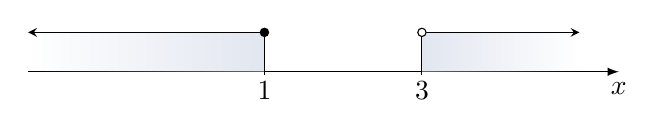
\begin{tikzpicture}
		\nlAxisX{-2}{5}
		\nlnuminf{3}{o}
		\nlinfnum{1}{c}
	\end{tikzpicture}	
	\end{Verbatim}
	
	gives us
	
	\medskip

	
	\begin{center}
		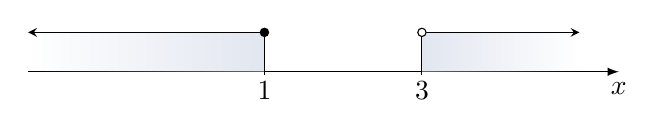
\begin{tikzpicture}
			\nlAxisX{-2}{5}
			\nlnuminf{3}{o}
			\nlinfnum{1}{c}
		\end{tikzpicture}
	\end{center}
	
	This time, there are a few optional inputs, the full commands are like this:
	
	\begin{Verbatim}[gobble=1,xleftmargin=5mm]
		\nlnuminf[1]{number}[2]{o or c}[3]
		\nlinfnum[1]{number}[2]{o or c}[3]
	\end{Verbatim}

	\begin{itemize}
		\item in [1] you can put options like different colours or patters used;
		\item in [2] you can substitute the number for a letter or an exact representation of the number, don't put it in math environment!;
		\item in [3] you can change the height of the interval, which is \(0.5\si{\centi\meter}\) by default.
	\end{itemize}


	Let's try some of these options:
	
	\begin{Verbatim}[gobble=1,xleftmargin=5mm]
	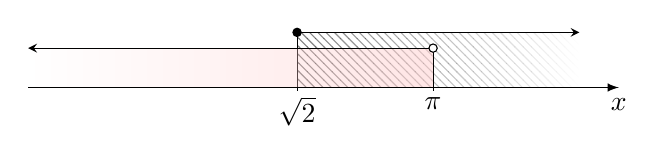
\begin{tikzpicture}
		\nlAxisX{-2}{5}
		\nlnuminf[pattern=north west lines]{1.4142}[\sqrt{2}]{c}[.7]
		\nlinfnum[red!20]{3.1416}[\pi]{o}
	\end{tikzpicture}	
	\end{Verbatim}
	
	
	\begin{center}
		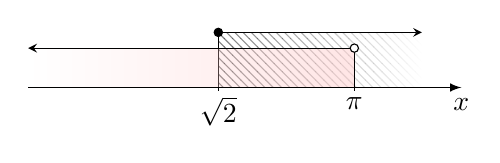
\begin{tikzpicture}
			\nlAxisX{-1}{4}
			\nlnuminf[pattern=north west lines]{1.4142}[\sqrt{2}]{c}[.7]
			\nlinfnum[red!20]{3.1416}[\pi]{o}
		\end{tikzpicture}
	\end{center}


\newpage
	
The second group of intervals, works with a single command:

\begin{itemize}
	\item \verb*|\nlnumnum|
\end{itemize}

and, since it uses two numbers, we have four mandatory inputs: the numbers and the instruction of closed or open. It works like this:


\begin{Verbatim}[gobble=1,xleftmargin=5mm]
	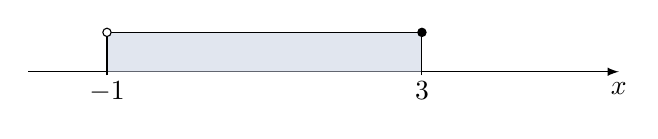
\begin{tikzpicture}
		\nlAxisX{-2}{5}
		\nlnumnum{-1}{o}{3}{c}
	\end{tikzpicture}
\end{Verbatim}
	
	\begin{center}
		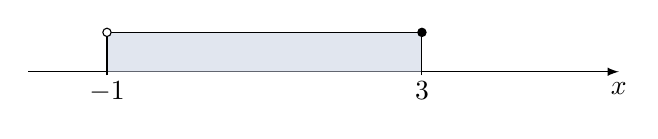
\begin{tikzpicture}
			\nlAxisX{-2}{5}
			\nlnumnum{-1}{o}{3}{c}
		\end{tikzpicture}
	\end{center}
	
As with the previous commands, there are a few options, this time we have one more which allows us to change what is shown in the second number:


\begin{Verbatim}[gobble=1,xleftmargin=5mm]
	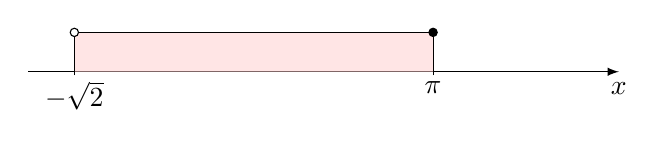
\begin{tikzpicture}
		\nlAxisX{-2}{5}
		\nlnumnum[red!20]{-1.4142}[-\sqrt{2}]{o}{3.1416}[\pi]{c}
	\end{tikzpicture}
\end{Verbatim}


\begin{center}
	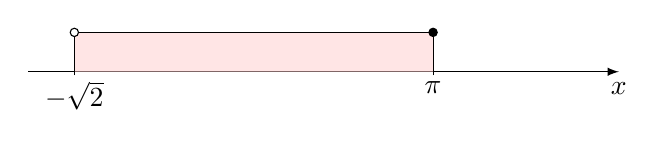
\begin{tikzpicture}
	\nlAxisX{-2}{5}
	\nlnumnum[red!20]{-1.4142}[-\sqrt{2}]{o}{3.1416}[\pi]{c}
\end{tikzpicture}
\end{center}


\section{Conclusion}

This is a really simple package (my first attempt at a package) but one that, I hope, can help you draw stuff like:

\begin{center}
	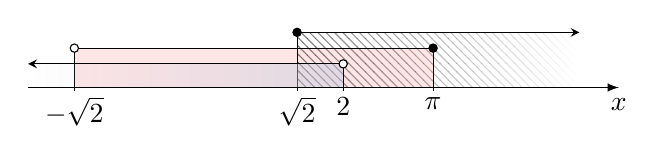
\begin{tikzpicture}
		\nlAxisX{-2}{5}
		\nlnumnum[red!20]{-1.4142}[-\sqrt{2}]{o}{3.1416}[\pi]{c}
		\nlnuminf[pattern=north west lines]{1.4142}[\sqrt{2}]{c}[.7]
		\nlinfnum{2}{o}[.3]
	\end{tikzpicture}
\end{center}

somewhat quickly and easily. By the way, the instructions for this are:

\begin{Verbatim}[gobble=1,xleftmargin=5mm]
	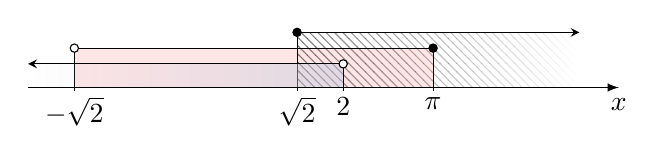
\begin{tikzpicture}
		\nlAxisX{-2}{5}
		\nlnumnum[red!20]{-1.4142}[-\sqrt{2}]{o}{3.1416}[\pi]{c}
		\nlnuminf[pattern=north west lines]{1.4142}[\sqrt{2}]{c}[.7]
		\nlinfnum{2}{o}[.3]
	\end{tikzpicture}
\end{Verbatim}


\end{document}